\documentclass{beamer}
\usetheme{Madrid}
\usecolortheme{default}

\title{Naive Utility Calculus}
\author{Joseph Low}
\date{August 2025}

\AtBeginSection[]{
  \begin{frame}
  \frametitle{Table of Contents}
  \tableofcontents[currentsection]
  \end{frame}
}

\begin{document}

\frame{\titlepage}

\begin{frame}
\frametitle{Table of Contents}
\tableofcontents
\end{frame}

\section{Introduction}
\begin{frame}
\frametitle{Introduction}
\vfill
\begin{center}
\fcolorbox{blue}{white}{\parbox{0.8\textwidth}{\centering\Large How do we make sense of other people's behavior?}}
\end{center}
\vfill

\pause

\begin{itemize}
    \item<2-> Why did you sleep late last night?
    \pause
    \item<3-> Why did you sign up for this course?
    \pause
    \item<4-> Why did you choose to eat out instead of cooking?
\end{itemize}
\end{frame}

\begin{frame}
\frametitle{Naive Utility}
\begin{center}
\Large $\text{Utility} = \text{Rewards} - \text{Costs}$
\end{center}
\vspace{0.5cm}
\begin{itemize}
    \item There is empirical support that humans intuitively use utility-based reasoning to make sense of other people's behavior
\end{itemize}
\vspace{0.5cm}
\begin{center}
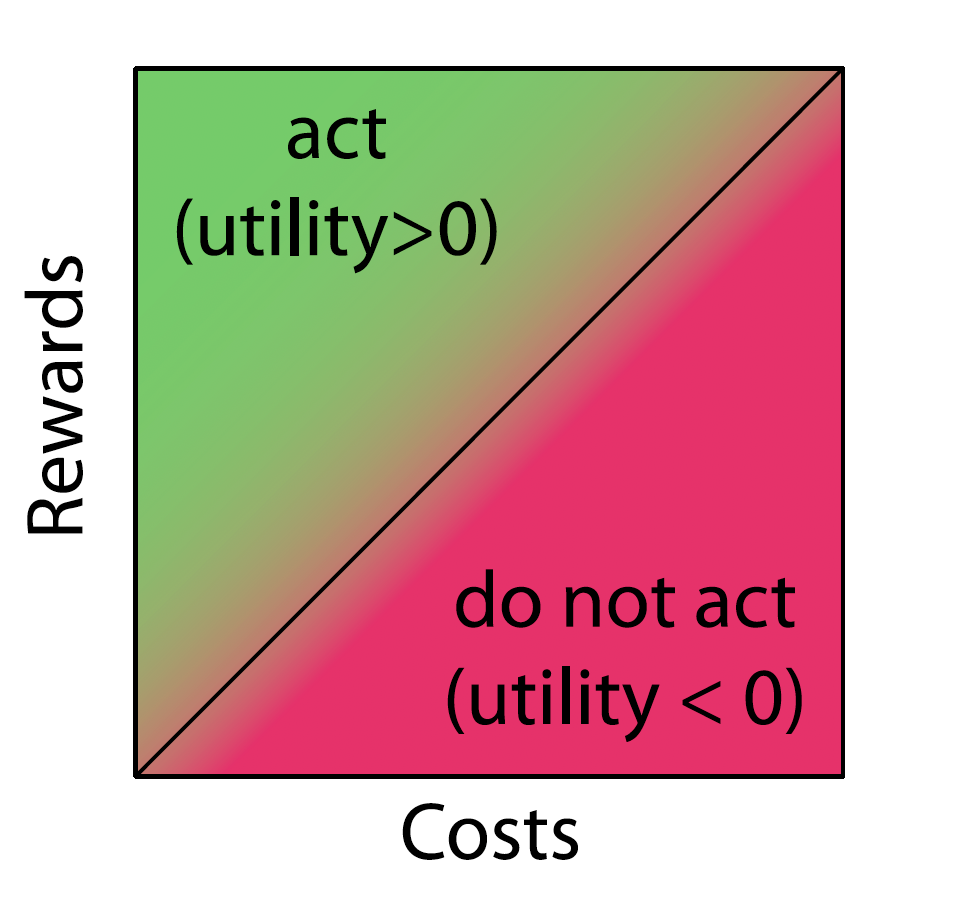
\includegraphics[width=0.4\textwidth]{utility1.png}
\end{center}
\end{frame}

\begin{frame}
\frametitle{Naive Utility Calculus}
\begin{center}
\Large $U(p, o) = R(o) - C(p)$
\end{center}
\vspace{0.5cm}
\begin{itemize}
    \item $U(p, o)$: utility expected from acting according to plan $p$ to reach outcome $o$
    \item $R(o)$: subjective reward the agent expects from outcome $o$
    \item $C(p)$: subjective cost of executing plan $p$
\end{itemize}
\end{frame}

\begin{frame}
\frametitle{Caveats}
\begin{itemize}
    \item \textbf{Descriptive, not normative:} This is not about how people \textit{should} make decisions (economic utility theory)
    \item \textbf{How we actually operate:} This describes how we \textit{intuitively} make sense of other people's behavior
    \item People don't explicitly compute utilities when they act - this is the cognitive framework we use to understand others
\end{itemize}
\end{frame}

\begin{frame}
\frametitle{Utility and Efficiency}
\begin{center}
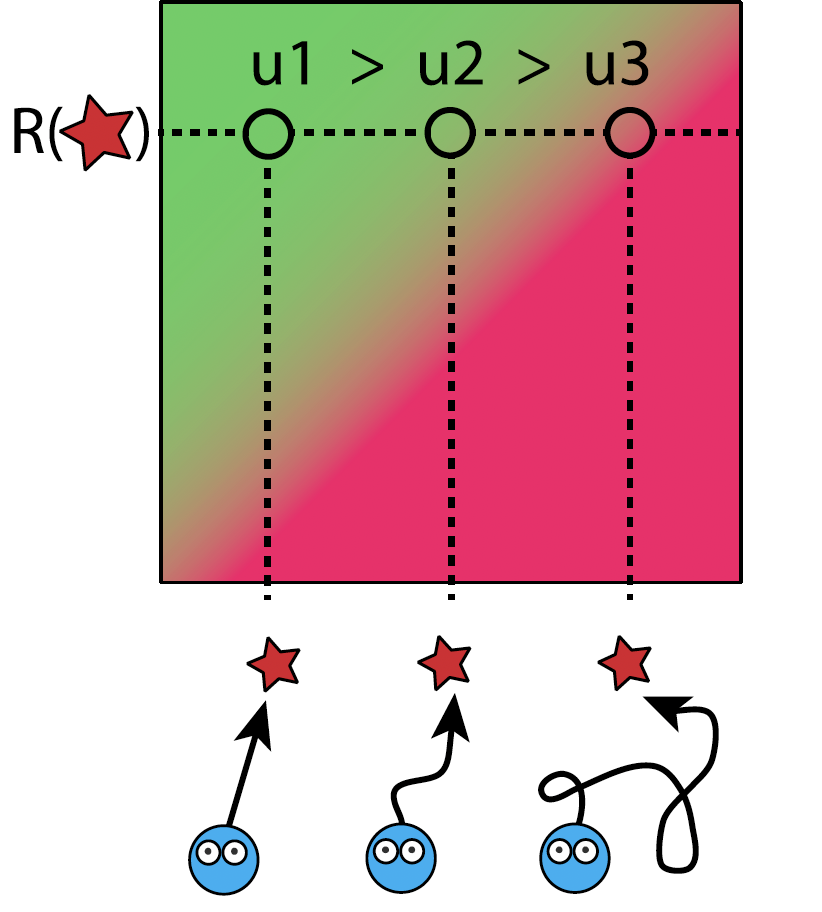
\includegraphics[width=0.3\textwidth]{utility2.png}
\end{center}
\vspace{0.3cm}
\begin{itemize}
    \item More efficient paths are less costly and therefore produce higher utilities
    \item When agents act, they will fulfill their goals as efficiently as possible to maximize utility
\end{itemize}
\end{frame}

\begin{frame}
\frametitle{Graded Preference Inference}
\begin{itemize}
    \item [Content to be added]
\end{itemize}
\end{frame}

\begin{frame}
\frametitle{Costs Vary Across Agents}
\begin{itemize}
    \item [Content to be added]
\end{itemize}
\end{frame}

\begin{frame}
\frametitle{Rewards Vary Across Agents}
\begin{itemize}
    \item [Content to be added]
\end{itemize}
\end{frame}

\section{Related Work}
\begin{frame}
\frametitle{Inverse Decision-Making}
\begin{itemize}
    \item [Content to be added]
\end{itemize}
\end{frame}

\begin{frame}
\frametitle{Inverse Planning}
\begin{itemize}
    \item Inferring goals and preferences from observed actions
    \item Often modeled using Markov Decision Processes (MDPs)
    \item Agent state transitions and reward functions
    \item [Additional content to be added]
\end{itemize}
\end{frame}

\begin{frame}
\frametitle{Research Questions}
\begin{itemize}
    \item [Content to be added]
\end{itemize}
\end{frame}

\section{NUC Computational Framework}

\begin{frame}
\frametitle{Hierarchical Mind Model}
\begin{center}
\begin{tabular}{|c|c|c|}
\hline
\textbf{Level} & \textbf{Component} & \textbf{Observable?} \\
\hline
4 & \textcolor{blue}{Desires} (Reward functions) & \textcolor{red}{No} \\
\hline
3 & \textcolor{blue}{Goals} (World states) & \textcolor{red}{No} \\
\hline
2 & \textcolor{blue}{Intentions} (Goal sequences) & \textcolor{red}{No} \\
\hline
1 & \textcolor{green}{Actions} (Behaviors) & \textcolor{green}{Yes} \\
\hline
\end{tabular}
\end{center}

\vspace{0.5cm}
\begin{center}
\Large $\downarrow$ \textbf{Inference Direction} $\uparrow$
\end{center}
\end{frame}

\begin{frame}
\frametitle{Generative Process}
\begin{center}
\begin{tabular}{c c}
\colorbox{blue!20}{\parbox{2.5cm}{\centering Desires \\ (Rewards)}} & \\
$\downarrow$ & + Costs \\
\colorbox{green!20}{\parbox{2.5cm}{\centering Goals}} & \\
$\downarrow$ & Utility Max \\
\colorbox{yellow!20}{\parbox{2.5cm}{\centering Intentions}} & \\
$\downarrow$ & Observable \\
\colorbox{red!20}{\parbox{2.5cm}{\centering Actions}} & \\
\end{tabular}
\end{center}
\end{frame}

\begin{frame}
\frametitle{MDP Planning per Goal}
\begin{center}
\textbf{Goal: Reach Object A}

\vspace{0.3cm}
$V^*(s) = \max_a \sum_{s'} P(s'|s,a)[R(a,s) - C(a,s) + \gamma V^*(s')]$

\vspace{0.5cm}
\textbf{Policy:} $p(a|s) \propto \exp(\sum_{s'} P(s'|s,a)V^*(s')/\alpha)$

\vspace{0.5cm}
Each goal $\rightarrow$ Separate MDP $\rightarrow$ Efficient path
\end{center}
\end{frame}

\begin{frame}
\frametitle{The Inference Problem}
\begin{center}
\begin{tabular}{c c c}
\colorbox{blue!20}{\parbox{2.5cm}{\centering \textbf{Hidden} \\ Costs \& Rewards}} 
& $\longrightarrow$ & 
\colorbox{red!20}{\parbox{2.5cm}{\centering \textbf{Observed} \\ Actions}} \\
& Forward & \\
& $\longleftarrow$ & \\
& \textcolor{red}{Bayesian Inference} & \\
\end{tabular}

\vspace{0.8cm}
$p(C,R|A) \propto p(A|C,R) \cdot p(C,R)$
\end{center}
\end{frame}

\begin{frame}
\frametitle{Two Types of Rationality}
\begin{center}
\begin{tabular}{|l|c|c|}
\hline
\textbf{Type} & \textbf{What} & \textbf{Formula} \\
\hline
Rational Choice & Intention selection & $p(I|C,R) \propto \exp(U(I)/\beta)$ \\
\hline
Rational Action & Efficient execution & $p(A|I)$ via MDP policy \\
\hline
\end{tabular}

\vspace{0.8cm}
\textbf{Likelihood:} $p(A|C,R) = \sum_I p(A|I) \cdot p(I|C,R)$
\end{center}
\end{frame}

\section{Experiments}
\begin{frame}
\frametitle{Experimental Setup}
\begin{itemize}
    \item [Content to be added]
\end{itemize}
\end{frame}

\begin{frame}
\frametitle{Experiment 1}
\begin{itemize}
    \item [Content to be added]
\end{itemize}
\end{frame}

\begin{frame}
\frametitle{Experiment 2}
\begin{itemize}
    \item [Content to be added]
\end{itemize}
\end{frame}

\begin{frame}
\frametitle{Experiment 5}
\begin{itemize}
    \item [Content to be added]
\end{itemize}
\end{frame}

\section{Discussion}
\begin{frame}
\frametitle{Discussion}
\begin{itemize}
    \item Summary of key points
    \item Main takeaways from this presentation
    \item Future directions and next steps
    \item Questions and discussion
\end{itemize}
\end{frame}

\end{document}